% Implementation/Contributions of Whirlpool
\chapter{Implementating Whirlpool}\label{implwhirlpool}
\begin{figure*}[h!]
    \centering
    \begin{subfigure}
        %\centering
        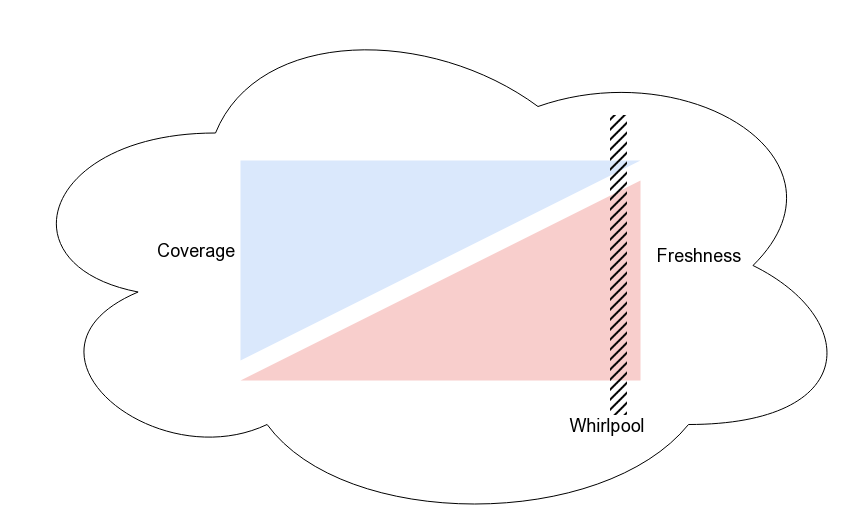
\includegraphics[width=3in, height=2.0in]{../media/crawler/whirlpool-crawl-order.png}
    \end{subfigure}
    ~
    \begin{subfigure}
        %\centering
        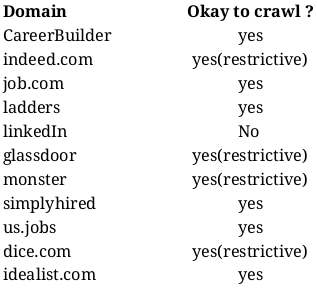
\includegraphics[width=3in, height=2.0in]{../media/crawler/whirlpool-seed-set.png}
    \end{subfigure}%
    \caption{Whirlpool seed set \& its crawl ordering policy}
    \label{fig:missionchar}
\end{figure*}

\noindent
Whirlpool is a continuous, topical crawler(section \ref{covfresh}) that never terminates by itself, figure \ref{fig:missionchar}. The focus is to maximize freshness over coverage of content crawled from given seeds. The seeds are active job portals which serve as a perfect candidates to continuously monitor and revisit already visited pages. This is done without overhauling the seed servers by implementating the url frontier scheme (section \ref{scheme}).

\pagebreak